%%%%%%%%%%%%%%%%%%%%%%%%%%%%%%%%%%%%%%%%%%%%%%%%%%%%%%%%%%%%%%%%%%%%%%%%%%%%%%%%
%2345678901234567890123456789012345678901234567890123456789012345678901234567890
%        1         2         3         4         5         6         7         8
% THESIS CHAPTER

\chapter{The task}
\label{chap:task}
\ifpdf
    \graphicspath{{EvaluationTask/Figures/PNG/}{EvaluationTask/Figures/PDF/}{EvaluationTask/Figures/}}
\else
    \graphicspath{{EvaluationTask/Figures/EPS/}{EvaluationTask/Figures/}}
\fi


% short summary of the chapter
An evaluation task must be set based on which the algorithms are analysed,
evaluated and compared.

\section{Design} 
\label{sec:design}
The design of the evaluation task follows the general structure for an algorithm
targeted towards utilising a large-scale database. In includes taking a query
song and creating pairwise comparisons of it with any song from a song database.
The similarity score of each pair is then calculated using a cover song
identification algorithm and an ordering is created. The pair with the highest
similarity includes the database song that the algorithm has identified to be
most similar to the query song (and potentially its cover version). 

As a song database the evaluation task uses several music datasets. Each dataset
contains sets of different versions of a song. The unique identifier that
combines all versions of a single song is called a \textit{clique}. For
instance, the original version song 'Take On Me' by the Norwegian band A-ha and
its cover version created by the American punk rock artist MxPx are in the same
clique named \textit{Take On Me}. Each dataset is split into a symbolical
\textit{train} and \textit{test} sets. The train portion of the songs is
initialised as a song database, while each of the tracks in the test set is used
as a query song. During the split it is ensured that there is at least one song
from each clique in both the train and test set, so that for every query song a
cover ready to be identified is found in the song database.

The task results are produced through a benchmark written using Python
\cite{python} and storing the song database into a MongoDB \cite{mongodb}
instance. Figure \ref{fig:bencharch} shows a high-level architecture diagram of
the benchmark, which could help understand the general design of the evaluation task.

\begin{figure}[H]
    \centering
    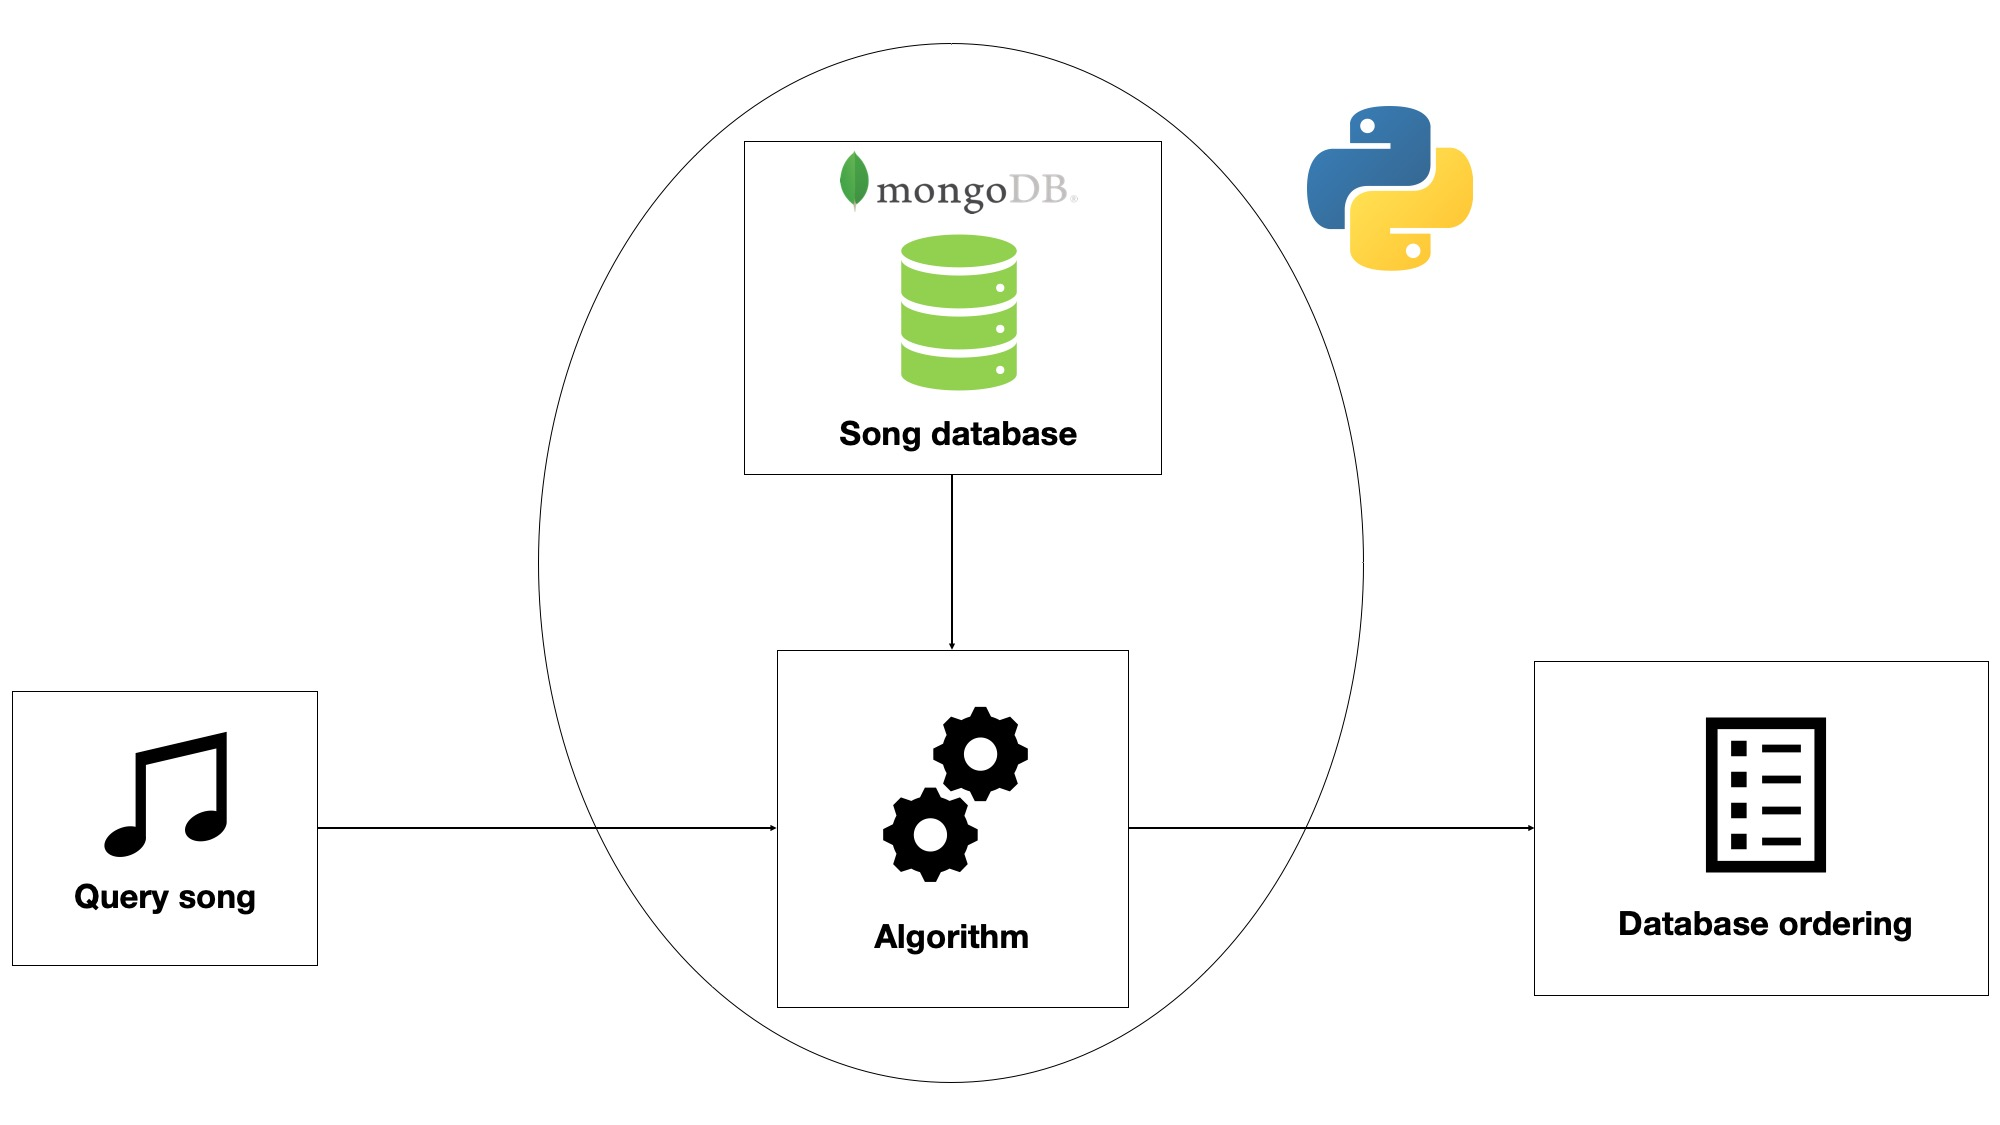
\includegraphics[width=\textwidth]{EvaluationTask/benchmark_architecture_2.jpg}
    \captionof{figure}[Benchmark architecture diagram]{Benchmark architecture diagram}
    \label{fig:bencharch}
\end{figure}

\section{Evaluation methods and metrics} 
\label{sec:evalmethods}
All algorithms are evaluated using metrics adapted from the MIREX \textit{Cover
Song Identification} competition format. The benchmark implements the following
measurements:
\begin{itemize}
    \item \textit{mean rank (MR)} of the position of a true cover (a song from
    the same clique as the query song) in the database ordering produced by an
    algorithm
    \item \textit{mean reciprocal rank (MRR)} of the position of a true cover in
   the database ordering produced by an algorithm
   \item covers identified in the \textit{Top-K} positions of the database
   orderings for all songs, where $K$ is a number 
   \item covers identified in the \textit{Top-P} percentile of the database
   orderings for all songs, where $P$ is a number 
\end{itemize}

\section{Datasets used for evaluation} 
\label{sec:datasets}
One of the main challenges in the project was the lack of appropriate datasets,
therefore some of the datasets are self-curated using my personal music
collection. The algorithms were evaluated using the following datasets:
\begin{itemize}
    \item \textit{covers80} - a widely used by MIR researchers consisting of 80
    cliques and 164 songs \cite{covers80}. Contains original compositions and
    cover versions of them.
    \item \textit{live\_dataset} - a self-curated dataset consisting of 70
    cliques and 145 songs. Contains original compositions and professionally
    recorded, mixed and mastered live performances of them.
    \item \textit{yt\_dataset} - a self-curated dataset consisting of 16 cliques
    and 32 songs. Contains original compositions and live performances of them
    recorded from an audience perspective using a smartphone.
\end{itemize}

A list of all songs in each dataset is provided in the Appendix, as well as in
the benchmark source code GitLab repository \cite{gitlabrepo}.
